%% ****** Start of file apstemplate.tex ****** %
%%
%%
%%   This file is part of the APS files in the REVTeX 4 distribution.
%%   Version 4.1r of REVTeX, August 2010
%%
%%
%%   Copyright (c) 2001, 2009, 2010 The American Physical Society.
%%
%%   See the REVTeX 4 README file for restrictions and more information.
%%
%
% This is a template for producing manuscripts for use with REVTEX 4.0
% Copy this file to another name and then work on that file.
% That way, you always have this original template file to use.
%
% Group addresses by affiliation; use superscriptaddress for long
% author lists, or if there are many overlapping affiliations.
% For Phys. Rev. appearance, change preprint to twocolumn.
% Choose pra, prb, prc, prd, pre, prl, prstab, prstper, or rmp for journal
%  Add 'draft' option to mark overfull boxes with black boxes
%  Add 'showpacs' option to make PACS codes appear
%  Add 'showkeys' option to make keywords appear
%\documentclass[aps,prb,preprint,superscriptaddress,showkeys,endfloats]{revtex4-1}
%\documentclass[aps,prb,preprint,superscriptaddress,showkeys]{revtex4-1}
\documentclass[aps,prl,reprint,superscriptaddress,showkeys]{revtex4-1}
\usepackage{amsmath}
\usepackage{color}
\usepackage{graphicx}
\usepackage{dcolumn}
\usepackage{verbatim}
\newcolumntype{d}{D{.}{.}{-1}}





\begin{document}




%\title{Fully parallel methods for calculation of partition functions for systems with known number of states with application to crystalline Li$_2$OHCl and Li$_2$OHBr}
\title{B$_L$ENDER algorithm for naturally parallelizable calculation of energy density of states}

\author{Jason Howard}
\affiliation{Materials Science Division Argonne National Lab}
\email{jdhoward@anl.gov}

\date{\today}

%\begin{abstract}
%\input{abstract}
%\end{abstract}


\begin{acknowledgments}
\end{acknowledgments}
\begin{abstract}
In this work  an algorithm is proposed that calculates the energy density of states, this algorithm combines random sets with Wang and Landau importance sampling  and is naturally parallelizable. The algorithm is referred to as B$_L$ENDER, which is an acronym for B$_L$end Each New Density Each Round and  adjective for  how it was created and functions. The algorithm was developed for the purpose of working towards the goal of using first principles simulations, such as density functional theory, to calculate the partition function of disordered sub lattices in crystal materials. In this work  B$_L$ENDER  is tested with the 2d Ising model as an analogous system to the disorded cubic phase of the solid state lithium ion electrolyte Li$_2$OHCl. This was done in order to make a prediction of the  wall time necessary for B$_L$ENDER to evaluate the partition function of a 3$\times$3$\times$3 supercell of disordered cubic Li$_2$OHCl. This work also demonstrates that, during the simulation to calculate the energy density of states, linear averages of  order parameters can be made for each energy level. With these averages and the energy density of states the ensemble average of the order parameter can be determined at any temperature. 
\end{abstract}
\maketitle
For crystalline  materials  with disordered sub-lattices such as the Li ion solid state electrolyte  Li$_2$OHCl\cite{Hood, Goodenough, Schwering, Holzwarth_group, Song_Borodin} it is desirable to calculate from first principles methods the density of energy states $G(E_j)$. With the energy density of states the partition function,
\begin{equation}
\begin{split}
Z = \sum_{i}^{\Omega}e^{\frac{-e_i}{k_B T} }= \sum_{j}^{\Pi}G(E_j)e^{\frac{-E_j}{k_BT}} \;,
\end{split}
\end{equation}
can be  determined and from it many important thermodynamics properties such as the free energy, entropy, specific heat, and ensemble averages calculated. One method to solve this problem could be temperature dependent simulations involving the  Metropolis algorithm and histogram re-weighting techniques\cite{metropolis_equation_1953, landau_MC_simulations}.  Another algorithm called the  Wang and Landau algorithm\cite{WL_phys_rev_lett} has been developed which is temperature independent. An issue with these algorithms in use with first principles methods such as density functional theory is the large number of iterations needed which would require a prohibitively long wall time at the current performance power of computers.  In this paper a method is proposed that combines the use of random sets along with the importance sampling method of the Wang and Landau algorithm that is meant to work towards the goal of highly parallel importance sampling algorithms that mesh well with high performance computing architectures. The algorithm developed in this work is referred to as the ``B$_{L}$ENDER" (B$_{L}$end Each New Density Each Round) algorithm. The name ``B$_{L}$ENDER" functions as an  adjective as well as acronym which comes in part because how it blends the ideas of a random set and the Wang and Landau method, and also due to the nature of the algorithm iteratively blending histograms to produce a converged density of states.  The Wang and Landau method does have parallel versions, including  restricting random walkers to specific energy ranges or allowing the walkers to explore the entire space while periodically communicating with each other \cite{MP_Wang_Landau,P_imp_Wang_Landau, Hframe_Wang_Landau}.  B$_{L}$ENDER is natural to parallelize as it is based on a set of random walkers that each can explore the entire energy range. It is hoped that due to B$_{L}$ENDER being presented in the form of sets that the mathematics of set theory and real analysis can be used to analyze the algorithm and possibly further extended its capabilities from those presented in this work. 

  In a previous paper the notion of the master set $\{ \Sigma_i, e_i \}_\Omega $ of the $\Omega$ total configurations and energies was put forth. The master set refers to the actual configurations of the defined system. In practice the calculation of the energy density of states $G(E_j)$  may only be possible through randomly sampling the configuration space.  In a previous work it was shown that a properly scaled histogram of a uniformly sampled random set $\{ \Sigma_s, e_s \}_\mathcal{S}$ converges to the exact density of states $G(E_j)$ as the the number of samples $\mathcal{S}$ goes to infinity. The problem with this method is that if $\Omega$ is large, which it is for many problems,  then the computationally effort to achieve convergence is not feasible.  This work tackles this issue and produces an algorithm that is highly parallel in terms of the calculations of the energies  but also incorporates importance sampling such as in the Wang and Landau method.
   
The ``B$_{L}$ENDER" algorithm proposed in this work  is given as follows. It is noted that the following algorithm is in terms of producing a relative density of states $H(E_j)$. 

\begin{equation}
\begin{split}
&1.\hspace{0.125cm} H(E_j)^i ,\hspace{0.15cm}  \{\Sigma_{s},e_s\}_{\mathcal{S}}^i\\
&2. \hspace{0.125cm}\{\Sigma_{s},e_s\}_{\mathcal{S}}^i \rightarrow  \{\Sigma_{s}^{'},e_s^{'}\}_{\mathcal{S}}^i\\
&3. \hspace{0.125cm}H(E_j)^{Ii} = H(E_j)^i + \mathcal{H}(E_j, \{e_{s}^{'}\}_{\mathcal{S}}^i) \\
&4. \hspace{0.125cm} \Sigma_{s}^{i'}, e_s^{i'} \rightarrow \Sigma_{s}^{i+1},e_s^{i+1}   \hspace{0.125cm} P = \hspace{0.075cm} min (1, H(e_s)^{Ii}/H(e_s^{'})^{Ii})\\
& \hspace{0.125cm}else  \hspace{0.15cm} \Sigma_{s}^i, e_s^i \rightarrow \Sigma_{s}^{i+1}, e_s^{i+1}\\
&5. \hspace{0.125cm} H(E_j)^{i+1} = H(E_j)^{i} + C_o\mathcal{H}(E_j, \{e_s\}_{\mathcal{S}}^{i+1})\frac{H(E_j)^{Ii}}{\sum_j H(E_j)^{Ii} }\\
&6. \hspace{0.125cm} N = \sum_j H(E_j)^{i+1} \hspace{0.125cm}\\
& if \hspace{0.125cm} H(E_j)^{i+1}\frac{\Omega}{N}  < 1, \hspace{0.125cm}  H(E_j)^{i+1} =  \frac{N}{\Omega}
\end{split}
\end{equation}
Where  $H(E_j)^0 \equiv \mathcal{H}(E_j,\{e_s\}_{\mathcal{S}}^0)$ with $\mathcal{H}(E_j,\{e_s\}_{\mathcal{S}})$ being a histogram function that counts the number of energies $E_j$ in the set $\{e_s\}_{\mathcal{S}}$. In this work $\{\Sigma_{s},e_s\}_{\mathcal{S}}^0$  is a randomly(uniformly) drawn set from the configuration space $\{ \Sigma_i, e_i \}_\Omega $. In the second step  a random change is applied to each element of the sampled set $\{\Sigma_{s},e_s\}_{\mathcal{S}}^i$ to produced a ``perturbed" set $ \{\Sigma_{s}^{'},e_s^{'}\}_{\mathcal{S}}^i$ , for the Ising model this could be randomly flipping a spin. In the third step a histogram of the ``perturbed" set is added to the current estimate of the density of states $H(E_j)^i$ to produce an intermediary density of states $H(E_j)^{Ii}$. In the fourth step a random number is drawn between zero and one for every sampled configuration, if this number is less then the ratio of the intermediary density of states $H(e_s)^{Ii}/H(e_s^{'})^{Ii}$ then the perturbed configuration and energy  $\Sigma_{s}^{'i},e_s^{i'}$  goes to $\Sigma_{s}^{i+1},e_s^{i+1}$,  else the unperturbed configuration and energy $\Sigma_{s}^{i},e_s^i$  goes to $\Sigma_{s}^{i+1},e_s^{i+1}$. In the fifth step a histogram of the updated $\{ e_s \}^{i+1}_{\mathcal{S}}$ energies is made and added (blended) in to the current density of states $H(E_j)^i$   by multiplying  by a constant $C_{o}$(which affects the convergence properties) and the relative probability of each energy $E_j$ in the  intermediary density of states $H(E_j)^{Ii}$. In this work it was found a $C_{o}=\Omega$ was computationally efficient. The sixth step corrects for a systematic error of a energy having a density of state less than one, in principle for a discrete system a given energy should have a density of state of a least one.  After the algorithm is deemed to be complete it is necessary to re-normalize the iterated relative density of states $H(E_j)^f$ at the final iteration $f$ as follows, 
\begin{equation}
\begin{split}
&1. \hspace{0.125cm} A = \sum_jH(E_j)^f\\
&2. \hspace{0.125cm} G(E_j)\approx H(E_j)^f \frac{\Omega}{A} \;,
\end{split}
\end{equation}
to produce the properly normalized estimated value of $G(E_j)$. 

In this work the algorithm discussed is tested using the 2-d square zero field  Ising model with lattice dimension of even number\cite{exact_statistical,Onsager,Ising}.  The configurations $\Sigma_i$ and energies $e_i$ of the 2-d Ising model are inherently defined by the lattice site spin variables and coupling constant $J$. In a previous study uniform sampling was used with first principles simulations to approximate the partition function for a $2\times 2\times 2$ supercell  of Li$_2$OHCl. In going to just a $3\times 3\times 3$ the value of $\Omega$ would jump from $\sim1e7$ to  $\sim1e26$. So computing the partition function for the $3\times 3\times 3$ system of Li$_2$OHCl is completely intractable from uniform sampling. In this work a $10X10$ 2d-ising model with $\Omega \approx 1.3e30$ is used as an analogous system to predict the computational effort needed for the B$_L$ENDER algorithm to compute the partition function of a  $3\times 3\times 3$ supercell of Li$_2$OHCl.  The first test is a test to show the convergence of the algorithm in terms of the number of samples $\mathcal{S}$ and the number of iterations of the algorithm. To test the accuracy of the simulations the results will be compared to the exact result solved by Beale \cite{Beale_2d_ising}. The accuracy of the simulation will be determined by the average of errors given as, 
\begin{equation}
\begin{split}
 &\mathcal{E}(I,o) \hspace{0.1cm}= \hspace{0.1cm}< |\epsilon(E_j,I,o)| >_j\\
& = \hspace{0.1cm}  \frac{1}{\Pi} \sum_{j=1}^{\Pi}\frac{|\ln(G_{ex}(E_j))- \ln(G_{bl}(E_j,I,o))|}{\ln(G_{ex}(E_j))}\; 
 \end{split}. 
\end{equation}
\begin{figure}[h!]
(a)\hspace{0.1cm}average iterations to reach $\mathcal{E}=1\%$ vs $\mathcal{S}$\\
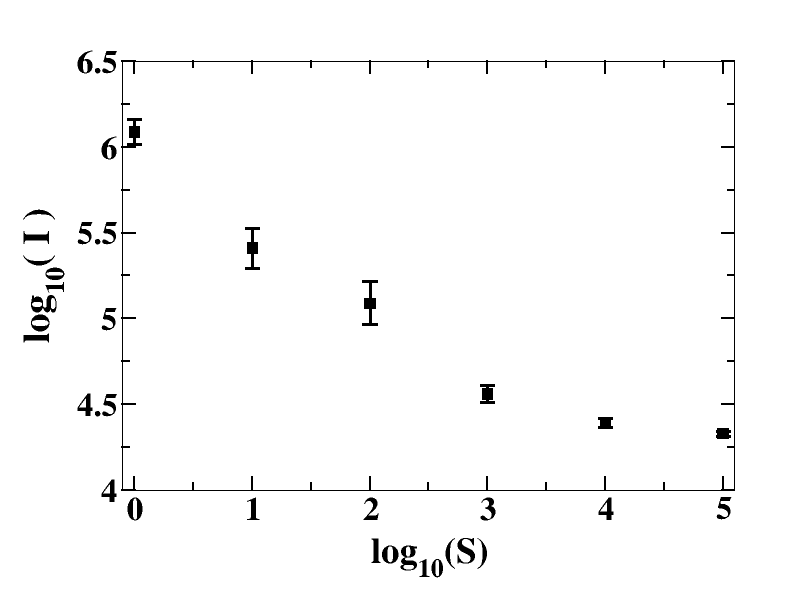
\includegraphics[width=7.5cm]{its_vs_S.png}\\
(b)\hspace{0.1cm}average iterations to find all energies vs $\mathcal{S}$\\
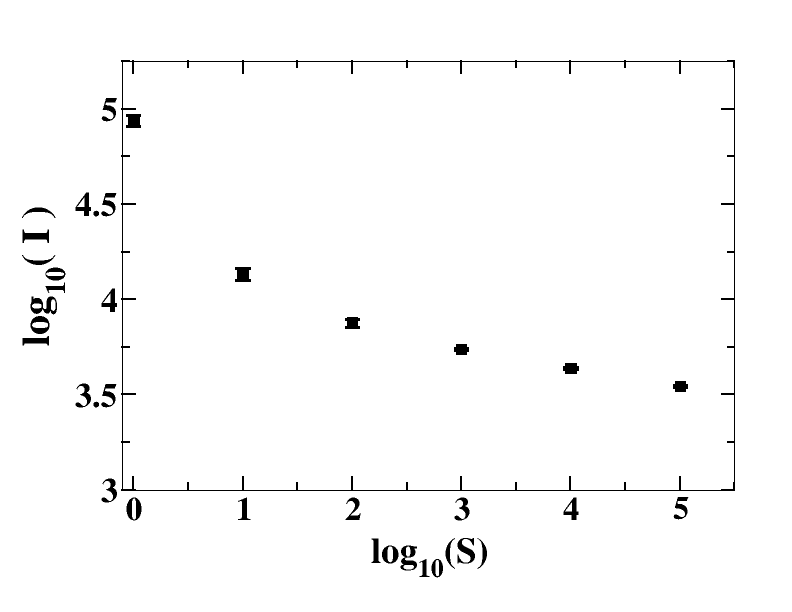
\includegraphics[width=7.5cm]{its_to_find.png}
\caption{\label{its_to}A $\log_{10}$ $\log_{10}$  plot of the average iterations $I$ to reach $\epsilon(I,o)=1\%$ vs the set size $\mathcal{S}$ (a) and the average number of iterations $I$ to find all of the energies vs the set size $\mathcal{S}$ (b). Error bars represent a linear propagation of the standard deviation of mean for $<I>_o$ in $\log_{10}$($<I>_o$). }
\end{figure}
Where $G_{ex}(E_j)$ is the exact density of states, $G_{bl}(E_j,I,o)$ is the calculated density of states  at iteration number $I$ from initial conditions and trajectory $o$, and $|\epsilon(E_j,I,o)|$ is the absolute value of the fractional error for a specific energy level. To test the algorithm on the 10$\times$10 Ising model, 144 individual calculations were performs at  $\mathcal{S}=$ 1, 10 ,100 , 1e3,  1e4, and 1e5. The number of iterations to find all the energies and the number of iterations to to reach $\mathcal{E}=1\%$ were recorded and averaged for each value of S. These results are shown in Fig \ref{its_to}  (a) and (b).  The plots show that the decrease in the number of iterations is not linear in including more samples $\mathcal{S}$ in the set, in the sense that there is an exponential like decay in the reduction in number of  iterations for an increase in samples.  

Something of interest to understand is some of the basic convergence properties of the error of the simulation. To test the the convergence of the algorithm in terms of iterations  36 simulations where done for  $\mathcal{S}=100$ for $1e9$ iterations. The average of the errors $<\mathcal{E}(I,o)>_o$ is shown in Fig  as a $\log_{10}$ $\log_{10}$  plot. The results show that the error appears to decrease approximately one order of magnitude for every order of magnitude increase in iterations.    

 Now from Fig \ref{its_to} (a) we could take $\mathcal{S}=100$  as an approximate optimal value to attempt a calculation of the density of states of cubic Li$_2$OHCl. In willing to accept $\mathcal{E}=10\%$ there is an approximate 10$\times$ reduction in the number of iterations. So for an accuracy of $\mathcal{E}=10\%$ that gives an approximate number of iterations  $\sim 1e4$, which if the calculations of the energies took 1 minute would take  7 days. On the other hand if the level of accuracy needed was to just find all the energies which from the figure is $\sim$ 8000 iterations the calculation would take 5.5 days for 1 minute calculations of the energies. Another point to make is that for calculation of the free energy of a disordered phase, it is not completely necessary to find all energy levels, which was demonstrated in a previous work. At the current level of computing power the calculation of the energies is greater than 1 minute so it would still require too large of a computational effort to make utilizing this algorithm on the Li$_2$OHCl system feasible but if Moore's law continues within a decade it may be a viable option. It must be stated that the estimation on the iterations required for the Li$_2$OHCl system is only meant for a coarse estimate and that a more detailed analogous model would be required to improve the prediction. The benefit of the square 2-d Ising model in this work is the availability of exact solutions. Aside from the difficulties in large supercells first principles simulations the algorithm could be used with first principles on smaller systems, with model Hamiltonians, or systems defined by a model potentials.  
\begin{figure}
(a)\hspace{0.1cm} $\mathcal{S}=$10\\
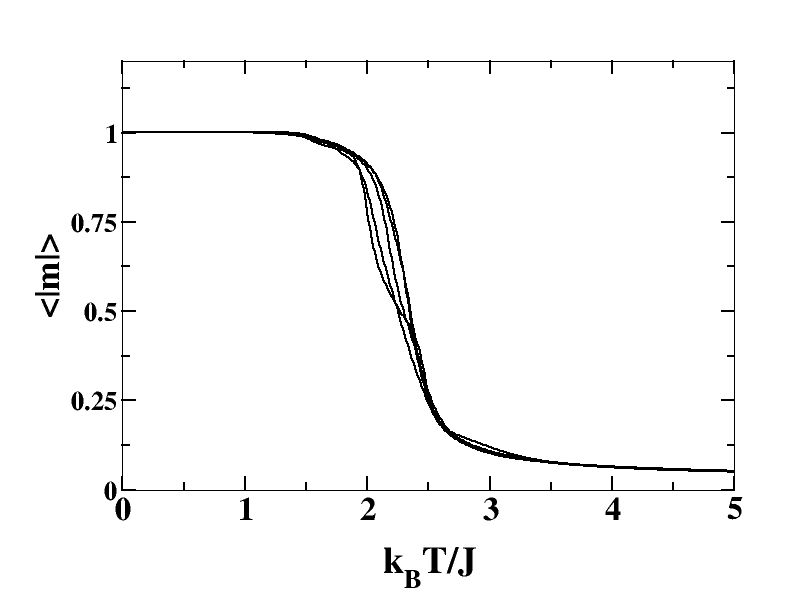
\includegraphics[width=7.5cm]{M_vs_T_S10.png}\\
(b)\hspace{0.1cm}$\mathcal{S}=$100\\
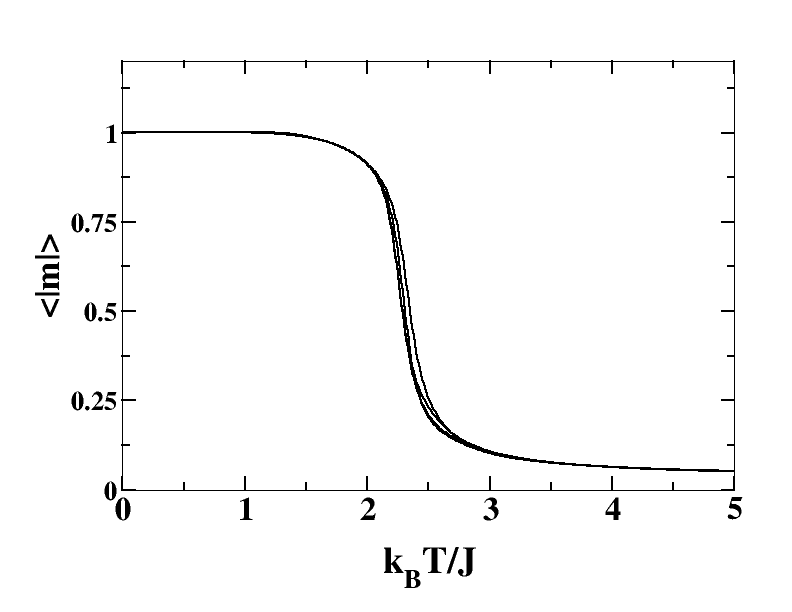
\includegraphics[width=7.5cm]{M_vs_T_S100.png}
\caption{\label{avg_mag} The ensemble averaged absolute value of the magnetization per lattice site calculated for a 26$\times$26 ferromagnetic Ising model  using $\mathcal{S}=$10 and $\mathcal{S}=$100 until $\mathcal{E}(I,o)=1\%$ shown in (a) and (b) respectively. Each plot displays five seperate calculations at each value of $\mathcal{S}$.  }
\end{figure}

 Once the energy density of states is obtained many important thermodynamic properties can be determined but it may be considered a draw back that ensemble averages of a general order parameter $a_i \equiv a(\Sigma_i)$ are not accessible.  It is shown in this work that this possible to achieve by considering the following equation, 
\begin{equation}
\begin{split}
&\langle a \rangle = \sum_i^{\Omega}a_i \frac{ e^{- \frac{e_i}{K_bT}  }}{Z} = \\
&\sum_j^{\Pi}<a_i>_{j}G(E_j)\frac{e^{-\frac{E_J}{K_bT} }}{Z} \; . 
\end{split} 
\end{equation}
Where $<a_i>_{j}$ is the linear/simple average of $a_i$ over all configurations with energy $E_j$. So if an average of the values visited  during the simulation is calculated then it may be possible to approximate ensemble averaged order parameters over the entire temperature range.  To test this the B$_L$ENDER algorithm was applied to a 26$\times$26 ferromagnetic Ising model with zero field with $\mathcal{S}=$ 10 and 100 to calculate the ensemble average of the absolute value of the magnetization per lattice site $\langle |m| \rangle$. In Fig \ref{avg_mag} (a) and (b) the results of five seperate simulations are shown for $\mathcal{S}=$ 10 and 100.  The results show that the known phase transition behavior of the ferromagnetic Ising model is well represented which indicates that this is a viable method for calculating ensemble averaged order parameters and that a larger value of $\mathcal{S}$ appears to reduce the variability between separate calculations.  This calculation is also evidence of B$_L$ENDER being applicable to larger systems, although this is still small compared to the 256$\times$256 model tested by Wang and Landau. 

In summary the presented algorithm in this work has shown its effectiveness in accurately determining the density of states for the 2D square zero field Ising model.  The simulations suggest that within a decade using B$_L$ENDER   it will be feasible on a state of the art super computer to calculate the partition function of a 3$\times$3$\times$3 135 atom model of disordered cubic Li$_2$OHCl using  density functional to a high level of accuracy. At the present time the algorithm should be suitable for first principles methods with smaller system sizes, with model Hamiltonians, or with models defined through model potentials. The algorithm shows promise for first principles methods in particular because the calculation of the energies can be done as individual job submissions to compute nodes managed by a script running on a head node. This work also demonstrated that if during the simulation to determine the energy density of states, linear/simple averages are made of order parameters for each energy level, then calculation of order parameters at any temperature is feasible. 
%\newcommand{\bibdir}{./}
\bibliography{Bib}
\bibliographystyle{unsrt}
\end{document}
